
\begin{figure}
    \centering
    \begin{subfigure}[t]{\fishfigwidth}
        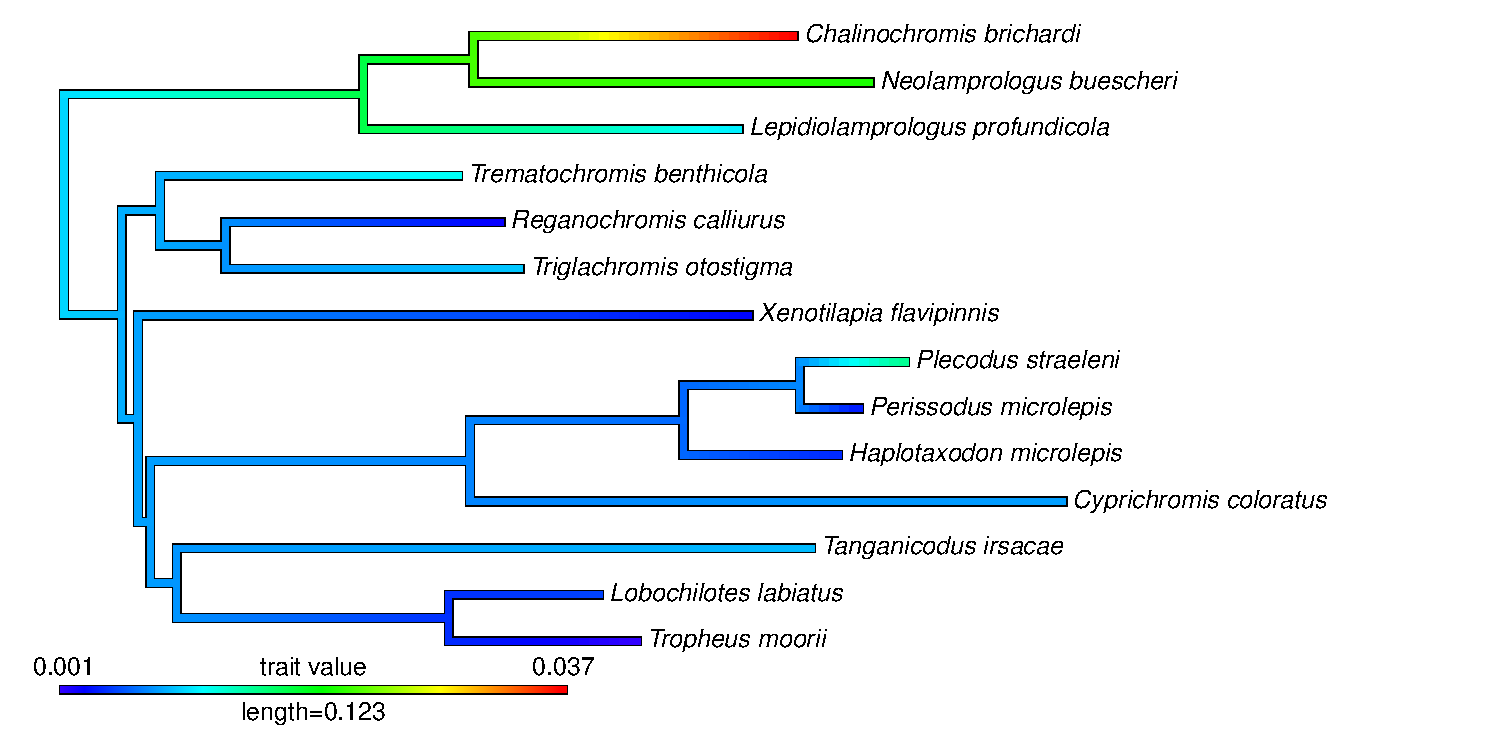
\includegraphics[width=\fishfigwidth]{FishPoo/figures/phylosig_heattree_highsig}
        \small
        \caption{{\tt CHALBRI1_1198} : Total abundance 0.14\%, Bloomberg's $K$=0.792551, Pagel's $\lambda$=0.640501, Moran's $\hat{I}$=0.330350, Abouheif's $C_{\mathrm{mean}}$=0.394249, 99\% identical to multiple species in the genus {\em Aeromonas}.}
    \end{subfigure}
    \begin{subfigure}[t]{\fishfigwidth}
        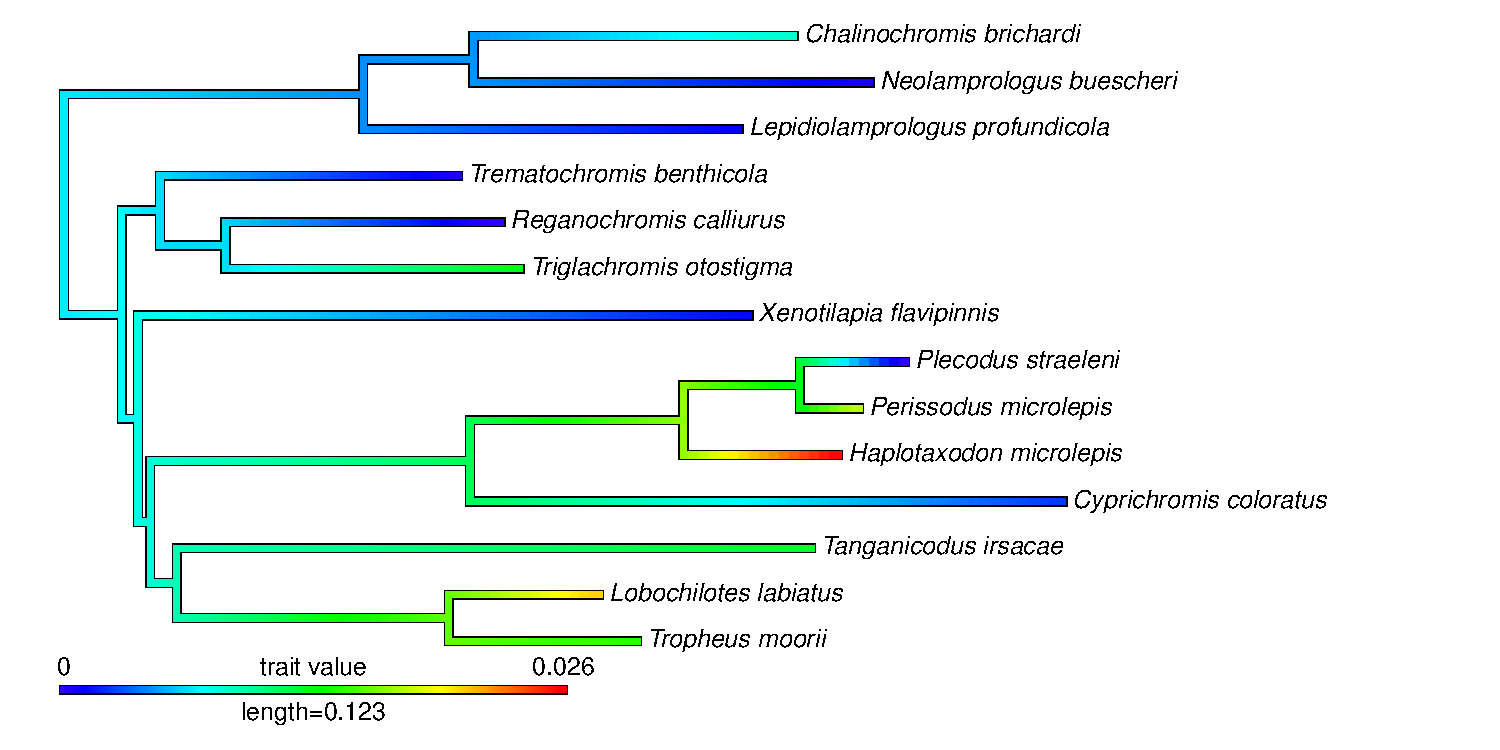
\includegraphics[width=\fishfigwidth]{FishPoo/figures/phylosig_heattree_lowsig}
        \small
        \caption{{\tt CHALBRI1_4931 : Total abundance 0.12\%, Bloomberg's $K$=0.425427, Pagel's $\lambda$=0.000047, Moran's $\hat{I}$=0.005716, Abouheif's $C_{\mathrm{mean}}$=0.046999}, 100\% identical to multiple the species in family Enterobacteriaceae.}
    \end{subfigure}
    \caption{Two examples of bacterial associations examined as traits of their hosts, one with high phylogenetic signal \textbf{(a)} and one with low phylogenetic signal \textbf{(b)}. However, the taxonomic assignments suggest that the second OTU may represent a more diverse group of organisms. If more than one of these organisms is present, then it is likely that each would have a different pattern of relationships with the host organisms. The sum of these patterns is likely to have a lower phylogenetic signal than any particular one of them. In principle, one could compensate for the different levels of diversity represented by different 16S sequences, but any such approach would require a relatively complete and unbiased database of microbial diversity. Unfortunately, such a database does not yet exist.}
    \label{fig:my_label}
\end{figure}